\subsection{Load driven threedimensional unconfined compression}
\label{subsec:Me5}

\subsubsection{Definition}
\label{subsubsec:Me5_def}

This example is similar to the previous one, differing in the kind of prescribed external loading: the calculation area undergoes traction boundary conditions (given surface stress) applied to the top of the model, while resulting deformation is unknown. In order to check out easily whether the simulated results correspond to the analytical solutions, the value of the prescribed axial stress coefficient $\sigma_{zz}$ on the top of the calculation area is chosen to have the same value as the resulting one obtained in the previous example.

\subsubsection{Solution}
\label{subsubsec:Me5_sol}

The finite element model has the same characteristics as the model in Sec.~\ref{subsec:Me4}. At the top of the model a constant conmpressive surface stress in axial direction with a value of 1.71$\times$10$^7$\,Pa is given as source term. The simulation with OpenGeoSys requires the input of the external load in terms of surface tractions as source term in $z$-direction at the single nodes of the stressed boundary. The displacement boundary conditions are the same as in the previous example except of the axial displacement on the top of the model. The used material parameters are shown in Tab.~\ref{Me_tab33}.


\begin{figure}[htbp]
\centering
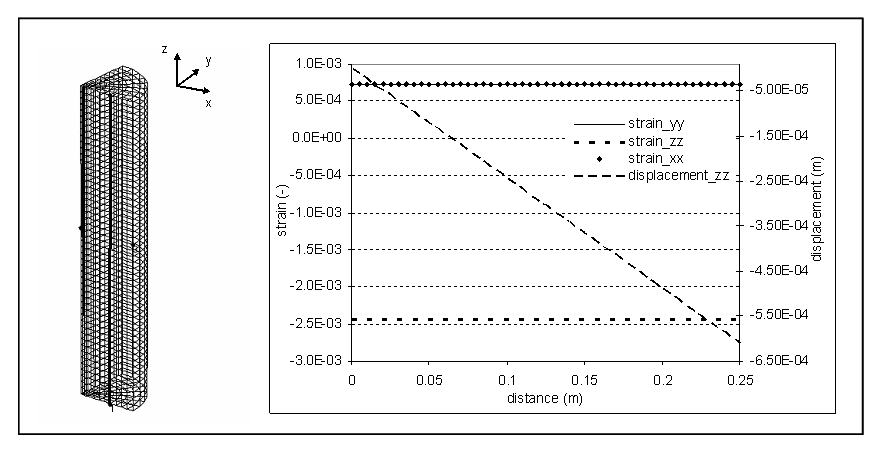
\includegraphics[width=0.9\textwidth]{PART_II/M/fig34.eps}
\caption{Strains and displacement in $z$-direction}
\label{Me_fig34}
\end{figure}

\subsubsection{Results}
\label{subsubsec:Me5_res}

The analytical solution and the numerical results are identical to that of the previous example. The calculated axial displacement as a result of the constant load on the top of the model is 6.1$\times$10$^{-4}$\,m. The numerical results that are shown in Fig.~\ref{Me_fig34} meet the analytical solutions exactly.
